\begin{frame}[fragile]{Tutorial: n-site states with MPS}

\begin{columns}

\begin{column}{4.5cm}

\begin{onlyenv}<1->
\begin{lstlisting}[language=JuliaLocal, style=julia, mathescape, basicstyle=\scriptsize\ttfamily]
  n = 30
  i = [Index(2, "S=1/2")
                  for j in 1:n]

  
  Zp = MPS(i, "Zp")

  maxlinkdim(Zp) == 1 # product state
\end{lstlisting}
\end{onlyenv}

\end{column}

\begin{column}{5.5cm}

\begin{onlyenv}<1-1>
\vspace*{-0.1cm}
$n$-site state \\
~\\
~\\
~\\
$|Z+Z+\dots Z+\rangle$ \\
~\\
~\\
\end{onlyenv}

\begin{onlyenv}<2->
\vspace*{0.0cm}
\begin{center}

\includegraphics[width=0.15\textwidth]{
  slides/assets/in.png
} \\
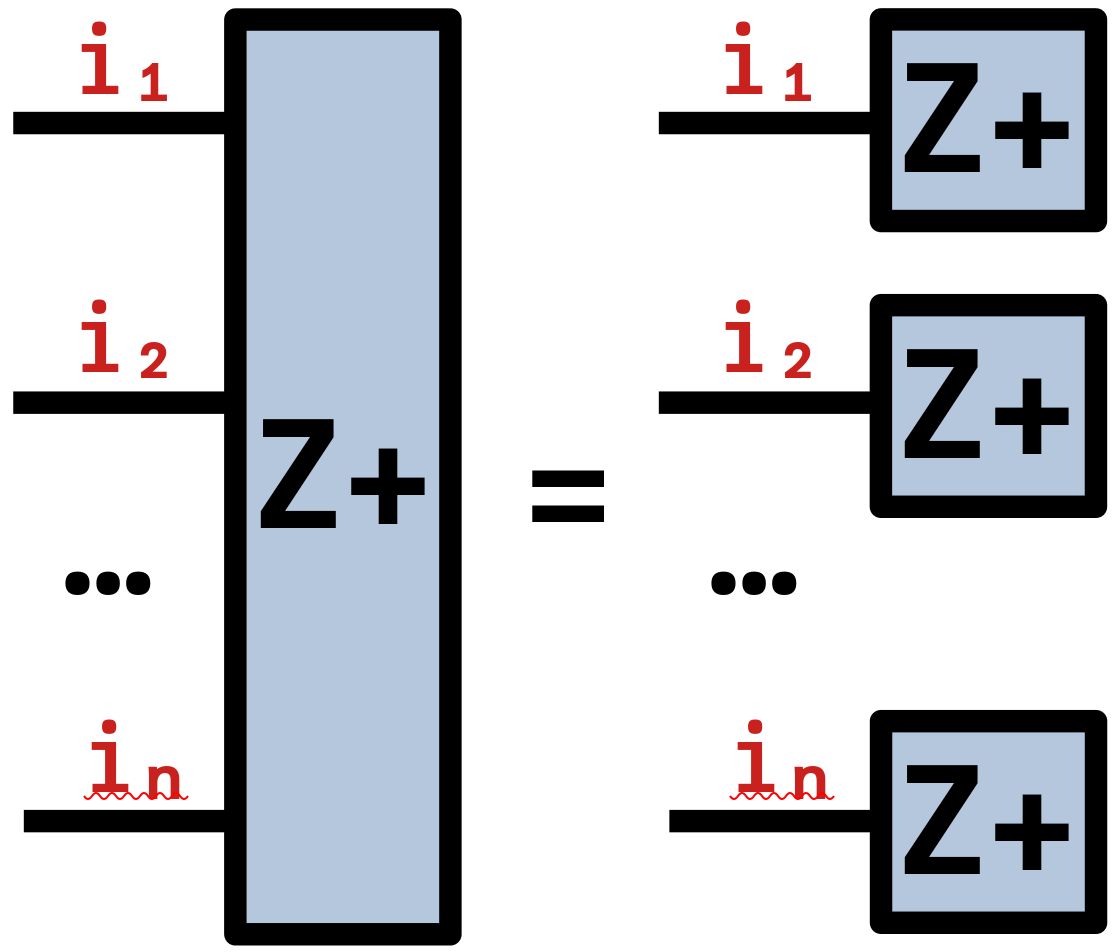
\includegraphics[width=0.5\textwidth]{
  slides/assets/Zpn.png
}
\end{center}
\vspace*{0.0cm}
\end{onlyenv}

\end{column}

\end{columns}

\end{frame}
